\chapter{Discussion}
\label{chp:discussion}

This chapter discusses the implications of our experimental results and their broader significance for 3D city modelling applications.

\section{Use Cases of FlatCityBuf}
\label{use_case_flat_city_buffer}

This section examines the most appropriate application scenarios for the FlatCityBuf format based on its demonstrated performance characteristics.

\subsection{Flexible Data Download}
\label{flexible_data_download}

Providing users with the ability to download specific data of interest represents one of the most valuable applications of 3D city models, particularly within open data initiatives. Existing services such as 3DBAG offer download functionality for CityJSON data in various formats including CityJSON, OBJ, and GeoPackage. However, these services typically constrain users to downloading predefined tiles rather than precisely the data matching their specific requirements.

\citet{fcb-web-demo} demonstrates a web application that enables users to download precisely the data they require. This implementation successfully showcases FlatCityBuf's capability to facilitate targeted data retrieval. Through its attribute indexing mechanism, users can download filtered datasets based on specific criteria, such as features exceeding 100 metres in height.

\subsection{Data Analysis}
\label{data_analysis}
\todo{this is not too convincing to me yet. Why mention CFD specifically here? most resources in CFD will not be affected by using FCB, maybe only a bit in the data preprocessing? (converting from FCB to CFD specific geometry enciding)
Mayber a more interesting use case is the 3DBAG generation pipeline, where we have different stages that need to read/write cjseq files, and I/O is actually one of the bottlenecks (eg in conversion from fcb to 3d tiles)}
As demonstrated by the performance benchmarks, FlatCityBuf excels in read operations compared to alternative data formats, making it particularly suitable for analysing large-scale datasets. Computational Fluid Dynamics in urban environments, for instance, requires processing substantial volumes of detailed geometric data. Such analyses typically demand significant memory and computational resources. FlatCityBuf can process these data more efficiently by leveraging its zero-copy capability.

The format also simplifies analytical workflows. Conventional approaches to large-scale data processing often require chunking data across multiple files, necessitating additional programming to manage file aggregation. In contrast, FlatCityBuf encapsulates data in a single file that can be efficiently loaded and accessed, even in web-based environments, streamlining analytical processes.

\section{Impact on Server Architecture}
\label{affect_on_server_architecture}

FlatCityBuf introduces significant opportunities for simplifying server architectures for 3D city model delivery.

\subsection{Traditional Server Architecture}
\label{traditional_server_architecture}

Conventional server architectures for 3D city models typically employ both application and database servers. For example, \citet{3dcitydb} utilises PostgreSQL or Oracle as the database server with PostgREST API \citep{postgrest} providing data access through its toolchain. Similarly, the 3DBAG API uses PostgreSQL as its database server and Flask (Python) as the application server.

In contrast, FlatCityBuf operates as a static file, requiring only a basic HTTP server such as Nginx for data distribution. This approach aligns with modern cloud service offerings, where providers like AWS S3 and Google Cloud Storage offer optimised solutions for serving static content.

\subsection{Cloud Architecture Advantages}
\label{cloud_architecture_achieved}

\subsection{Scalability}
\label{scalability}

Scalability presents a significant challenge in traditional server architectures. These systems typically employ Relational Database Management Systems (RDBMS) that often encounter scaling limitations. Common mitigation strategies include sharding and replication (horizontal scaling) or resource expansion (vertical scaling), both requiring additional computational, memory, and storage resources.

FlatCityBuf circumvents these challenges by functioning as a static file that can leverage cloud providers' inherent scalability and high availability infrastructure. This characteristic offers substantial benefits for applications built on 3D city model data. Service providers can host static FlatCityBuf files on standard servers, allowing unrestricted access for various use cases without implementing the rate-limiting mechanisms often necessary with traditional server architectures.

\subsection{Cost-effectiveness}
\label{cost_effectiveness}

FlatCityBuf contributes significantly to operational cost-effectiveness. Although precise server costs vary according to specific use cases, hosting static files through cloud service providers is generally substantially more economical than maintaining dedicated database and application servers.

\todo{add more description of comparison}
\begin{figure}[htbp]
  \centering
  \begin{subfigure}[b]{0.48\textwidth}
    \centering
    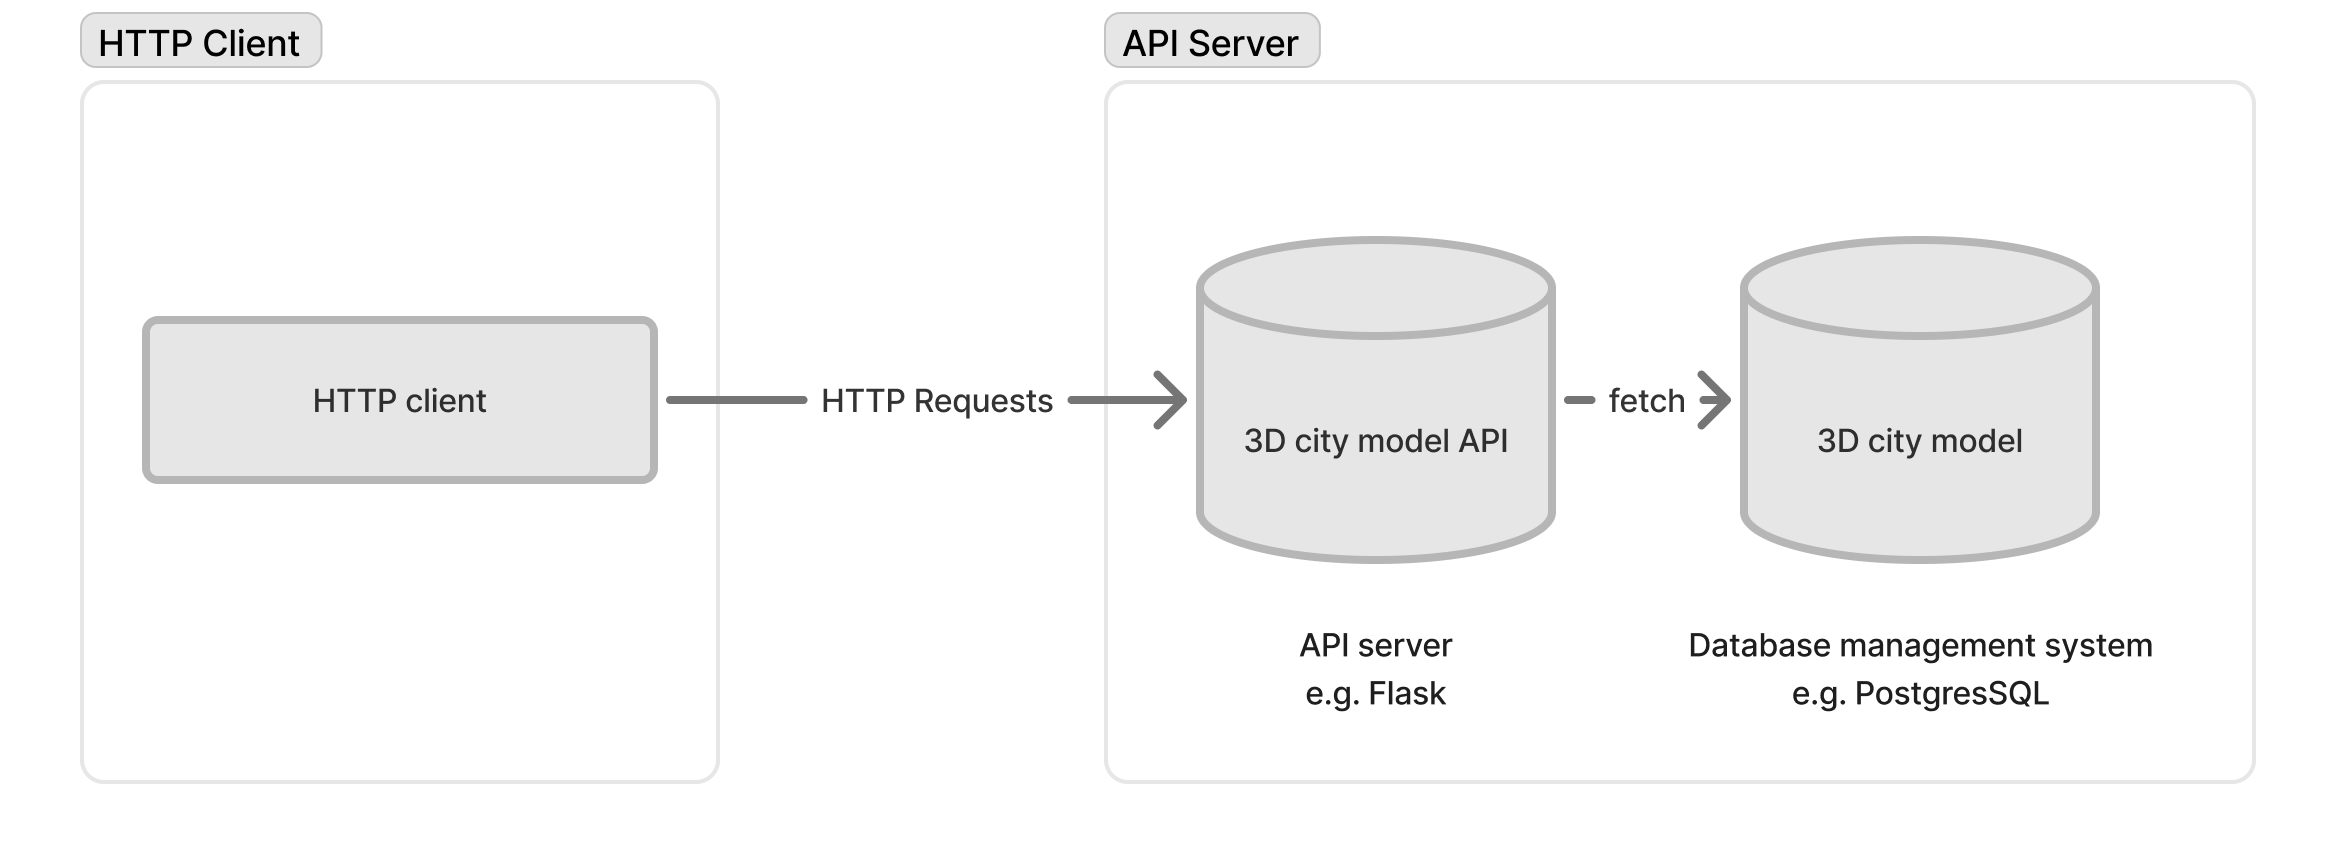
\includegraphics[width=\textwidth]{figs/discussion/server_architecture.png}
    \caption{Traditional server architecture with database and application servers}
    \label{fig:traditional_architecture}
  \end{subfigure}
  \hfill
  \begin{subfigure}[b]{0.48\textwidth}
    \centering
    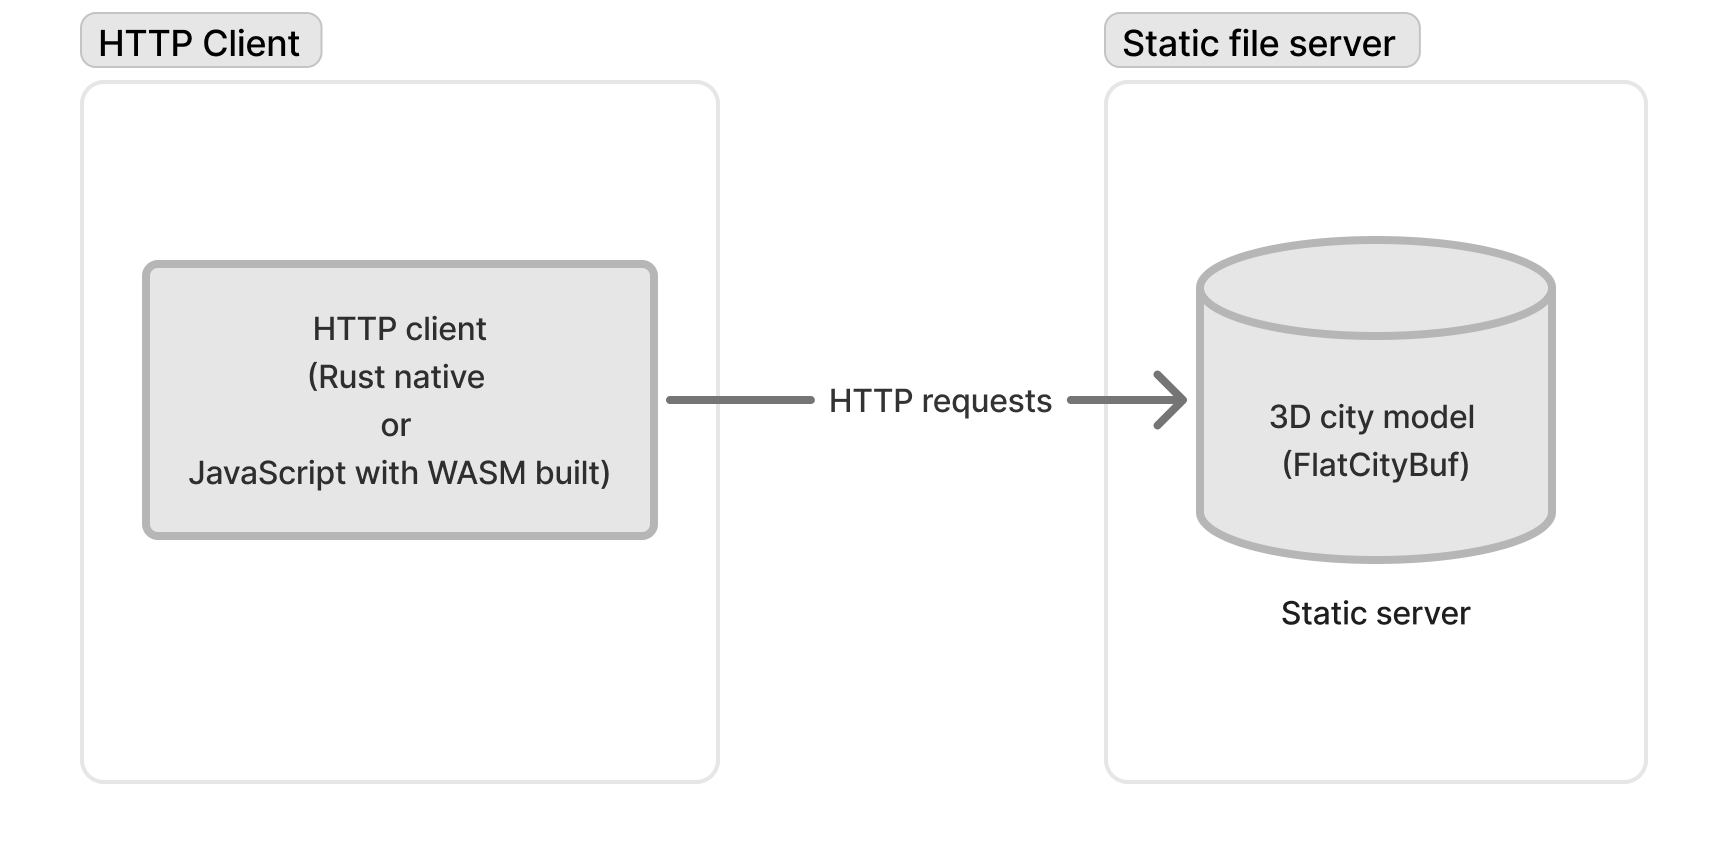
\includegraphics[width=\textwidth]{figs/discussion/server_architecture_fcb.png}
    \caption{Simplified FlatCityBuf architecture}
    \label{fig:fcb_architecture}
  \end{subfigure}
  \caption{Comparison between traditional and FlatCityBuf server architectures. The proposed method eliminates the need for complex database infrastructure by leveraging static file hosting with built-in spatial and attribute indices.}
  \label{fig:architecture_comparison}
\end{figure}

\section{Limitations}
\label{limitations}

Despite its advantages in simplicity, scalability, and cost-effectiveness, FlatCityBuf does present certain limitations that warrant consideration.

\subsection{Query Flexibility}
\label{flexibility_of_query}

While FlatCityBuf supports both spatial and attribute indexing, its query capabilities remain more constrained than those of specialised spatial database applications. Traditional approaches employing RDBMS with spatial indexing provide more comprehensive query functionality. For instance, 3DCityDB enables filtering by LoD, CityObject type, and various other parameters, whereas FlatCityBuf primarily supports attribute-based filtering. Similarly, regarding spatial functions, 3DCityDB can utilise the extensive spatial capabilities of PostGIS, while FlatCityBuf currently only implements bounding box queries. Consequently, FlatCityBuf is optimised for scenarios requiring relatively straightforward filtering conditions.

\subsection{Client-side Application Complexity}
\label{complexity_of_client_side_application}

Although FlatCityBuf simplifies server architecture, it introduces additional complexity in client-side applications, which must implement logic for loading and processing the format. By comparison, OGC API and equivalent Web API services adhere to standardised designs that can be utilised by any client application—whether accessed through command-line interfaces, browsers, or mobile applications. While FlatCityBuf supports cross-platform applications, it requires language-specific or platform-specific library implementations.

\subsection{Update Complexity}
\label{ease_of_update}

Zero-copy data formats like FlatCityBuf generally present challenges for data updates due to their relatively rigid structure. Fixed-size data types such as integers or floating-point numbers cannot be dynamically converted to alternative types. Furthermore, since the format contains immutable spatial and attribute indices, updating the data necessitates rewriting the entire file. This characteristic renders FlatCityBuf less suitable for frequently updated datasets, positioning it instead as an optimal solution for data analysis and efficient download services.
